
\documentclass[a4paper, 12pt]{article}

\usepackage[utf8]{inputenc}
\usepackage{amsmath}
\usepackage[]{amsfonts}
\usepackage[]{graphicx}

\title{CS231A Course Notes 6: \\Fitting and Matching}
\author{Andrew Chen}
\date{}

\renewcommand\emph{\textbf}

\begin{document}

\maketitle

\section{Introduction}
Previously, we have worked with mostly perfect data, where a solution for a model can typically be calculated outright.  However, in real-life situations, we typically do not have the privilege of working with such ideal data.  Noise, outliers, missing data, and intra-class variation are all complications that require us to take different approaches to choosing and parameterizing a model to describe our data.

In these lecture notes, we introduce the topic of fitting, in which we aim to choose a parametric model to describe our imperfect data, and to estimate that model's parameters.  We'll focus on three techniques commonly utilized in computer vision: least squares methods, random sample consensus (RANSAC), and the Hough transform.

\section{Least Squares Methods}

Least squares methods approximate the solution of overdetermined systems, which are systems with more equations than unknowns.  Least squares methods approach this by minimizing the sum of the squares of the residuals between the solution and the data.  We'll focus our discussion on linear least squares, which fit a line to the data by minimizing the sum of squared residuals.

We can model a line in slope-intercept form with $y = mx + b \implies y - mx - b = 0$.  Given a dataset of points $\mathcal{D} = \{(x_1, y_1), ..., (x_n, y_n)\}$, the least squares error is given by
\[
E(\mathcal{D}, m, b) = \sum_{(x, y) \in \mathcal{D}} (y - mx - b)^2
\]
We can convert this to a matrix representation.
\begin{align*}
E(\mathcal{D}, m, b) &= \sum_{(x, y) \in \mathcal{D}} (y - mx - b)^2 \\
&= \sum_{(x, y) \in \mathcal{D}} \left(y - \begin{bmatrix} x & 1 \end{bmatrix} \begin{bmatrix} m \\ b \end{bmatrix} \right)^2 \\
&= \left\| \begin{bmatrix} y_1 \\ \vdots \\ y_n \end{bmatrix} - \begin{bmatrix} x_1 & 1 \\ \vdots & \vdots \\ x_n & 1 \end{bmatrix} \begin{bmatrix} m \\ b \end{bmatrix} \right\| ^2 \\
&= \left\| \textbf{Y} - \textbf{X}h \right\|
\end{align*}
where $\textbf{Y} = \begin{bmatrix} y_1 & \hdots & y_n \end{bmatrix}^T$, $\textbf{X} = \begin{bmatrix} x_1 & \hdots & y_n \\ 1 & \hdots & 1 \end{bmatrix}^T$, and $h = \begin{bmatrix} m & b \end{bmatrix}^T$, where $h$ is our parameterization of the line.  Continuing our derivation,
\begin{align*}
&= (\textbf{Y} - \textbf{X}h)^T (\textbf{Y} - \textbf{X}h) \\
&= \textbf{Y}^T \textbf{Y} - 2(\textbf{X}h)^T\textbf{Y} + (\textbf{X}h)^T\textbf{X}h
\end{align*}
Now, we want to find an optimal $\hat{h}$ that minimizes $E(\mathcal{D}, h)$, such that $\hat{h} = {\arg \min}_h E(\mathcal{D}, h)$.  We can do this by solving for $h$ in $\frac{dE}{dh} = 0$.
\begin{align*}
& \frac{dE}{dh} = -2\textbf{X}^T\textbf{Y} + 2 \textbf{X}^T \textbf{X} h = 0 \\
\implies & \textbf{X}^T \textbf{X} h = \textbf{X}^T\textbf{Y} \\
\implies & \boxed{\hat{h} = (\textbf{X}^T \textbf{X} )^{-1}\textbf{X}^T\textbf{Y}}
\end{align*}

This is a closed-form solution for $\hat{h}$.  

$\hat{h}$ can also be solved for using singular-value decomposition (SVD).  We leave this derivation as an exercise for the reader.

\section{RANSAC}

\underline{Ran}dom \underline{sa}mple \underline{c}onsensus (RANSAC) is an iterative method to estimate parameters of a model.  It is designed to be highly robust against outliers and missing data (in fact, one interpretation of the algorithm is that of an outlier discriminator).  Intuitively, RANSAC works through a voting scheme, in which a large number of random samples from the data each ``vote'' for their optimal parameterization.  These votes can then be tallied up, and the parameterization receiving the most votes can be considered the best.

Before discussing the algorithm in more detail, we will set up some of the background and assumptions made by the model.  A fundamental assumption is that data consists of \textit{inliers} and \textit{outliers}.  Inliers are data whose distribution can be well-explained by some parameterization of the model, and outliers are data that cannot be well-explained, due to extreme noise or an incorrect understanding of the underlying distribution.  

Let $s$ be the smallest number of data points required to fit a model, and $N$ be the number of samples to be taken by RANSAC.  Then, the RANSAC algorithm operates as follows:
\begin{enumerate}
\item $s$ points are randomly sampled from the data set.
\item A model is fit to these $s$ sampled data points.
\item Each of the remaining data points in the data set is classified as an inlier or outlier based on the fitted model.
\item Steps 1-3 are repeated $N$ times, and the model producing the greatest number of inliers is considered the best model.
\end{enumerate}

Let's walk through the example of applying RANSAC to line fitting.

\begin{figure}[h!]
\centering
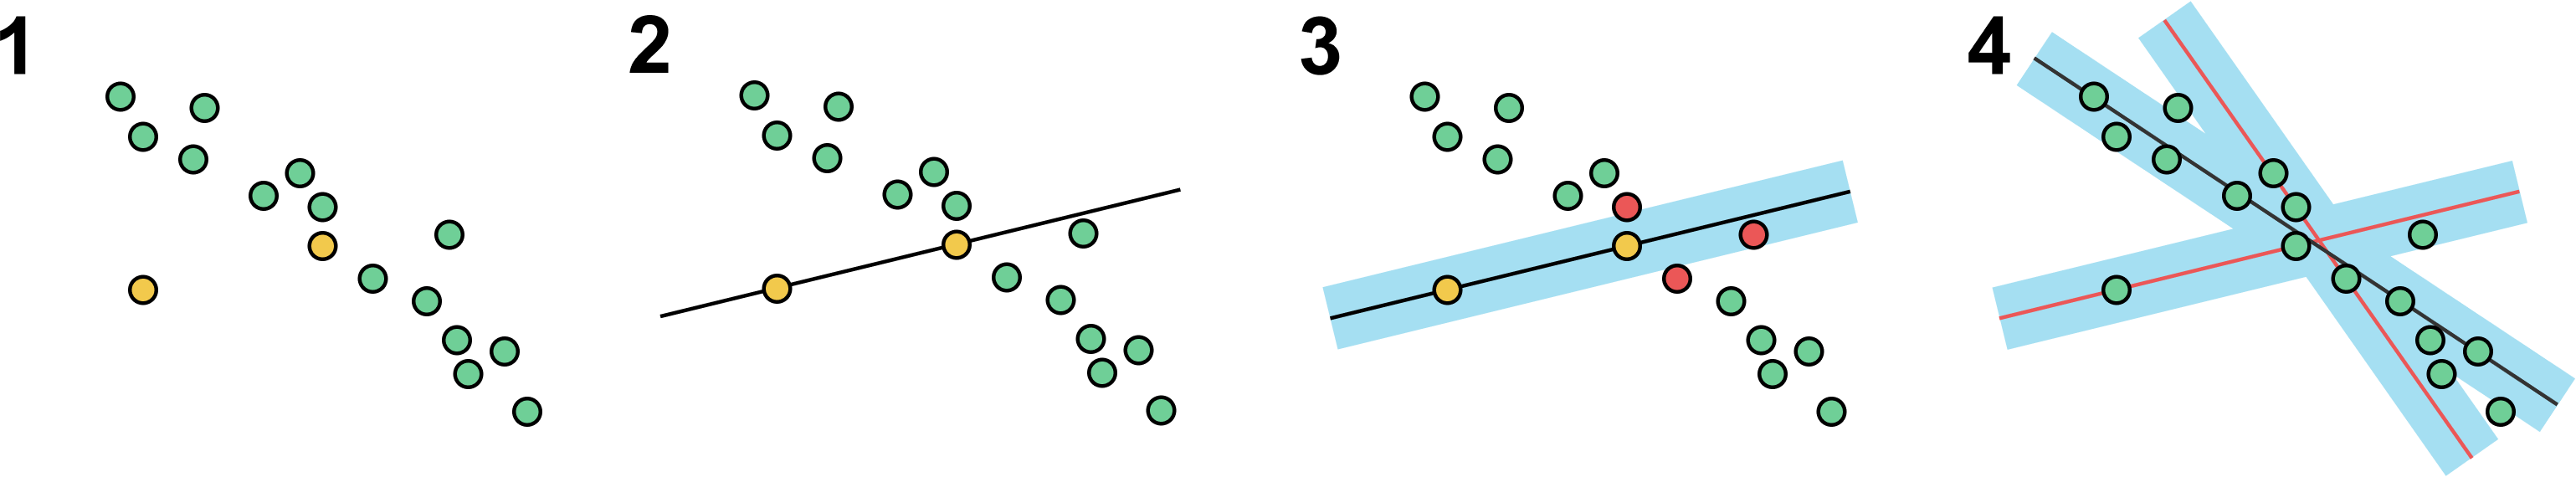
\includegraphics[width=0.95\textwidth]{figures/ransac_line}
\end{figure}
In (1), we sample $s = 2$ points, because two points are the minimum number required to fit a line.  In (2), we fit a line to these two points.  In (3), we classify each point in the remaining dataset as either an inlier (red) or outlier (green) based on the model.  Note that generally, the criterion for classifying a data point as an inlier or outlier is typically user-defined.  In this line fitting, the classification criterion for an inlier is whether the data point is within a certain distance from the line (blue area).  Finally, in (4), we repeat steps (1) to (3) $N = 3$ times, and choose the model that produces the greatest number of inliers.

For RANSAC to work well, we need to choose enough samples (large enough $N$) to result in a high probability that our best model is good.  We assume that a model is good if it is only fit to inliers.  Then, we can derive probabilistic bounds for RANSAC.  Specifically, we can derive the probability that at least one sample consists of all inliers, which would result in a good final model.  This is equivalent to calculating one minus the probability that all $N$ samples are contaminated with at least one outlier.

Let $p$ represent the probability that a point is an inlier, where $p = \frac{\textsf{inlier}}{\textsf{inlier} + \textsf{outlier}}$.  Then, the probability that any sample consists of only inliers is $p^s$, and the probability that any sample is contaminated with at least one outlier is $1 - p^s$.  The probability that all $N$ samples are contaminated is $(1 - p^s)^N$.  Then, the probability that at least one sample contains inliers only is given by one minus this value.  Therefore, the probability that we are able to acquire a good final model is
\[
1 - (1 - p^s)^N
\]
We can't control $p$ nor $s$, which are constrained by our dataset and our underlying problem representation, respectively.  However, we are able to change $N$ (at the cost of running time), to change the probability that we are able to acquire a good final model.  Let $p_\textsf{good}$ represent the probability that we are able to acquire a good final model from RANSAC.  Then,
\begin{align*}
& 1 - (1 - p^s)^N = p_\textsf{good} \\
\implies & (1 - p^s)^N = 1 - p_\textsf{good} \\
\implies & N = \log_{(1 - p^s)} (1 - p_\textsf{good}) \\
\implies & \boxed{N = \frac{\log(1 - p_\textsf{good})}{\log(1 - p^s)}} \\
\end{align*}
We see that we can directly calculate the number of samples required to achieve a certain $p_\textsf{good}$.

\section{Hough Transform}

The Hough transform is a fitting technique that uses a voting scheme.  It parameterizes representations of shapes and objects from imperfect data.  We will focus our discussion on the Hough transform's classical application of fitting a line to imperfect data.

Recall that a line can be parameterized by $m, n$, such that $y = mx + n$.  We want to find the best-fitting line for our data, which is parameterized by $m = m', n = n'$.

Normally when we interact with our data, we visualize them in the original space with $x$-$y$ axes.  However, we can also convert our representation to Hough space, which has $m$-$n$ axes.  A point $(x_i, y_i)$ in the original space will be converted into a line $y_i = m x_i + n$ in Hough space.  The line representations of colinear points transformed to Hough space will intersect at a unique point.  

\begin{figure}[h!]
\centering
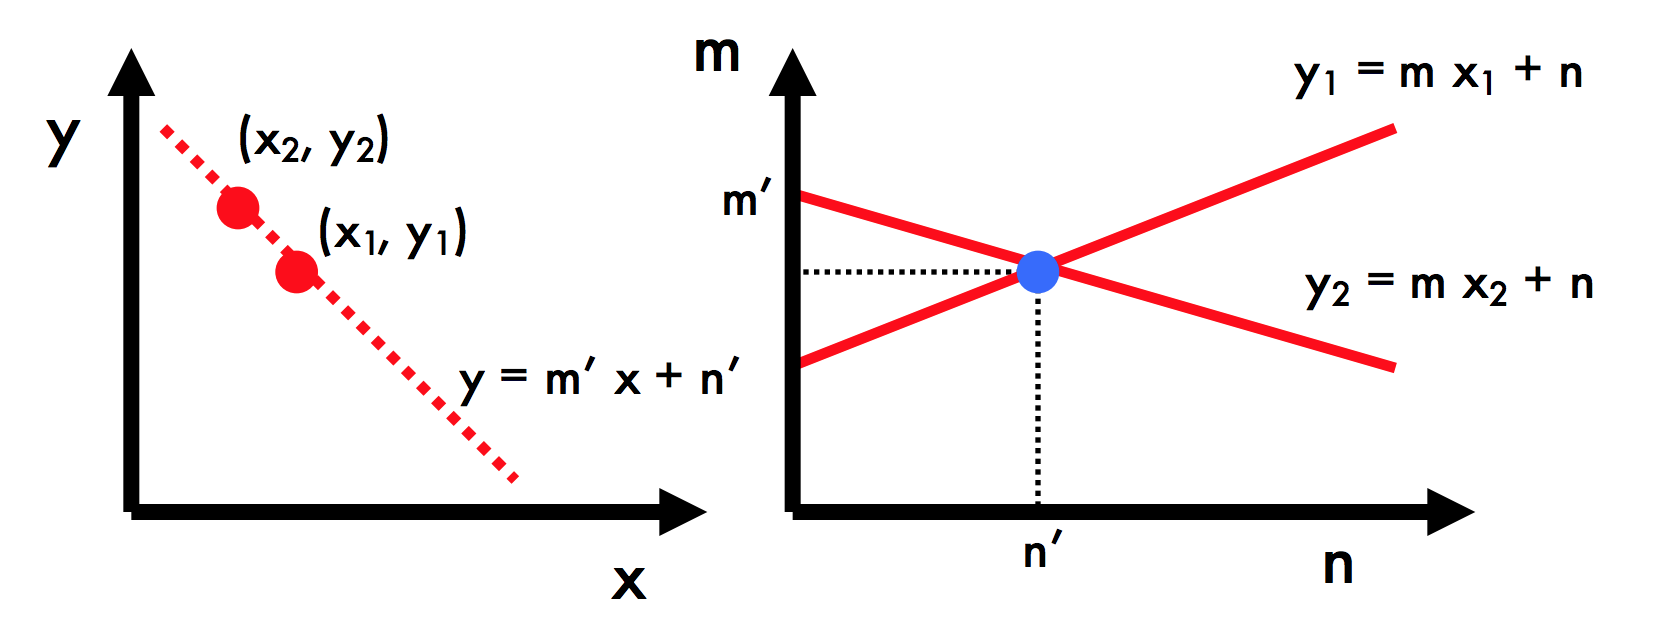
\includegraphics[width=0.8\textwidth]{figures/hough}
\caption{The transformation of data points from their original space to the Hough space.  The ideal parameterization of the best-fitting line for these two points is the intersection of the two lines in Hough space, which each represent a data point transformed to Hough space.  Figure from S. Savarese.}
\end{figure}

However, there is a problem with our current formulation --- the parameter space $[m, n]$ is unbounded.  $m \rightarrow \infty$ as lines tend towards vertical, and $n \rightarrow \infty$ as y-intercepts approach negative or positive infinity.  To address this issue, we forgo our slope-intercept representation of lines and instead use a polar representation.  Then, lines are parameterized by $\rho$ and $\theta$, such that $
\rho = x \cos \theta + y \sin \theta$.

\begin{figure}[h!]
\centering
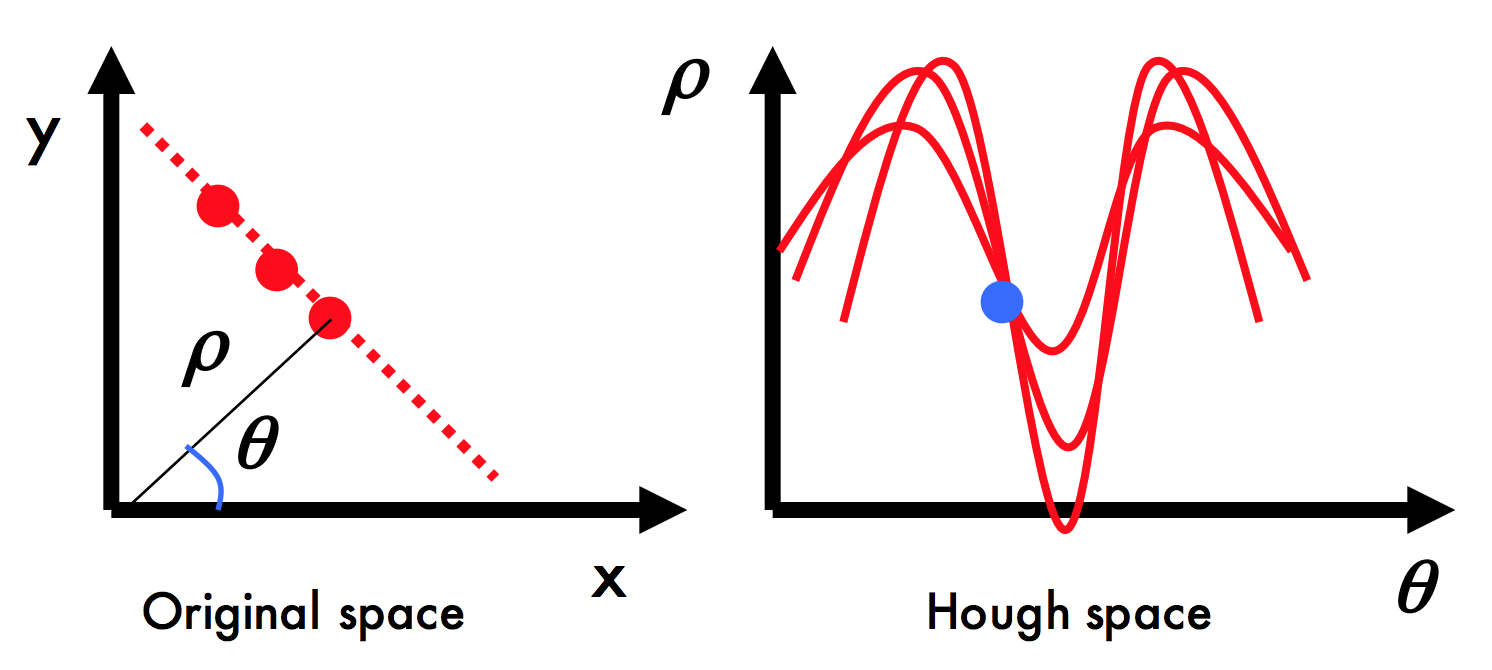
\includegraphics[width=0.75\textwidth]{figures/hough-polar}
\caption{Using a polar representation for the parameter space bounds the parameter space.  Figure from S. Savarese.}
\end{figure}

So far, our examples of the Hough transform have dealt with colinear points, which will all intersect at a single unique point in Hough space.  However, this becomes complicated with the addition of noise, which will almost always prevent us from observing an intersection of more than two data points.

We address this issue by introducing a voting scheme.  Intuitively, noise applied to colinear points will apply noise to their pairwise intersections in Hough space.  While this prevents these points from all intersecting at the same point in Hough space, their pairwise intersections will likely not be shifted that much.  As a result, we can introduce a grid over our parameter space and count the number of intersections within each cell.  Then, the cell with the greatest number of intersections will likely represent the ideal parameterization of the line (where $\rho, \theta$ are given by the coordinates of the center of the cell).

The Hough transform fitting method is relatively robust to random noise, which will typically not contribute consistently to any particular cell.  Furthermore, the technique is also robust to outliers, which will tend to vote for less popular cells.  However, the effectiveness of the Hough transform is dependent on the relationship between noise and cell size.  If the cell size is too small with respect to the noise, then intersections may be spread out over multiple cells, and a suboptimal cell elsewhere in the grid may come out with the most votes.  On the other hand, if the cell size is too large, then the precision of parameterization is greatly decreased. 

\end{document}